\documentclass[11pt,a4paper]{article}
\usepackage{polski}
\usepackage[utf8]{inputenc}
\usepackage{graphicx}
\usepackage{float}

\title{Laboratorium 4 - Sprawozdanie}
\author{Wojciech Makuch}

\begin{document}
\maketitle
\section{Zadanie}
Program framework benchmarkujacy dla zaimplentowanego algorytmu sortowania szybkiego opartego na strukturze typu lista.
\section{Realizacja}
Gotową implementacje listy skopiowano z repozytorium Sheaim/209226. Dodano metodę sortowania szybkiego \textsl{quicksort(int left, int right);} oraz uzupełniono kod o niezbędne metody, jak np \textsl{idz(int i);} pozwalająca odnieść się do konkretnego elementu listy. Dla algorytmu sortowania za piwot wybrano element środkowy sortowanej tablicy.

\section{Działanie}
Główna funkcja programu zawiera jedna pętle testującą algorytm. Uzyta funkcja \textsl{licz(dllist *obiekt, int N);} wypęłnia tablicę liczbami psełdolosowymi z zakresu 0-9 następnie mierzy i zwraca czas ich sortowania. Uzyskane wyniki program zapisuje do pliku o nazwie \textsl{pomiar\_czasu\_4.txt}

\section{Wyniki}
Z uzyskanych wyników wyrysowano przebieg funkcji pokazanej na Rysunku 1. Wynika z niego, że złożoność obliczeniowa takiego algorytmu wynosi $O(n^{2})$. Z teoretycznego punktu widzenia taka złożoność jest poprawna przy najgorszych założeniach(np. za duża lub za mała wartość piwota). Średnia złożoność obliczeniowa tego algorytmu wynosi $O(n logn)$.
\begin{figure}[t!]
\centering
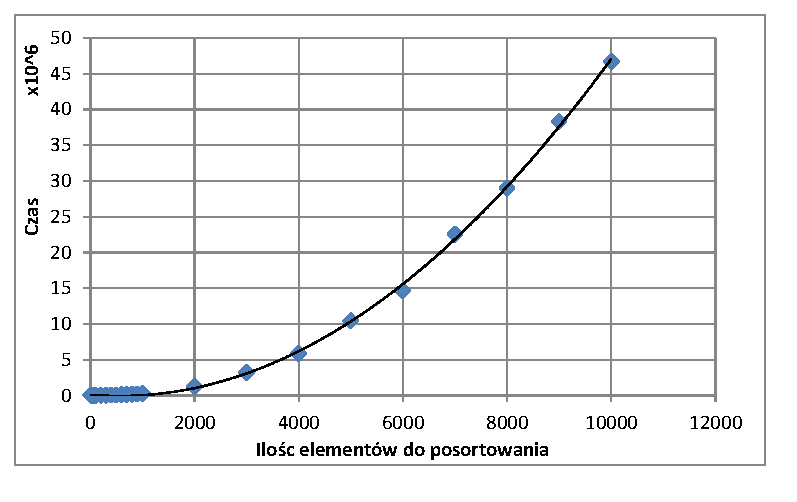
\includegraphics[scale=1]{wykr1.pdf}
\caption{Wykres złożoności obliczeniowej}
\label{fig:wykres1}
\end{figure}
\section{Komentarz}
Funkcja pomiaru czasu dla systemu Windows pobrana ze strony dr. J. Mierzwy. Program skompilowano w środowisku Code::Blocks. Do stworzonia wykresu posłużono się pakietem MS Excel, sprawozdanie napisano używając systemu \LaTeX.
\end{document}